\documentclass[usenames,dvipsnames]{beamer}

\usepackage{listings}
\usepackage{colortbl}% http://ctan.org/pkg/xcolor
\usepackage{tikz}
\usepackage{tikz-cd}
\usepackage{natbib}
\usepackage{bibentry}
\usepackage{color}
\usepackage{mathtools}
\usepackage{qtree}
\usepackage{rotating}
\usepackage[customcolors]{hf-tikz}
% \usepackage{tabularx}
\usetikzlibrary{positioning,chains,fit,shapes,calc}
\usetikzlibrary{shapes.geometric, arrows}
\usetikzlibrary{automata}

\usetheme{Pittsburgh}

\newcommand{\e}{\emptyset}
\newcommand{\req}[0]{\begin{turn}{90} $=$\end{turn}}

\newcommand{\emphasize}[1]{{\color[rgb]{1,0,0}#1}}
\newcommand{\emphasizeWhen}[2]{ {\color<#1>[rgb]{1,0,0} #2} }
\newcommand{\F}{\mathbb{F}}

\newcommand{\X}{{\!\!\color{red}\textbf{X}\!\!}}
\newcolumntype{d}{>{\columncolor[rgb]{0,0.5,0.5}}c}
\newcolumntype{P}{>{\columncolor[rgb]{0,0.5,0}}c}

\definecolor{light-gray}{gray}{0.95}

\title{Verifying Robustness of Programs Under Structural Perturbations}
\author{Clay Thomas and Jacob Bond}
\date{\today}

% \titlegraphic{
%   \includegraphics[width=0.4\textwidth]{Images/Purdue}
% }

\begin{document}

  % \bibliographystyle{alpha}
  % \nobibliography{robustness}

\begin{frame}
  \titlepage
\end{frame}

\begin{frame}[fragile]{Motivation}
  \begin{itemize}
    \item ``Sanity Checks''
    \vfill
    \item Functions invariant under order of list
    \begin{itemize}
      \item max, sum, sort
    \end{itemize}
    \vfill
    % mention bug finding
    \item Data structures with representing something else
    \item Invariance under value it represents
    \begin{itemize}
      \item binary search trees, heaps, hash sets
    \end{itemize}
  \end{itemize}
\end{frame}

% Not a great transition
\begin{frame}[fragile]{Lists -- Invariance under order}
  Given an array $a$
  \begin{itemize}
    \item Let $a_{swap}$ be $a$ with its first and second entry swapped
    \begin{itemize}
      \item $[ a[1], a[0], a[2], a[3], \ldots, a[n] ]$
    \end{itemize}
    \item Let $a_{rot}$ be $a$ rotated by $1$
    \begin{itemize}
      \item $[ a[1], a[2], a[3], \ldots  a[n], a[0] ]$
    \end{itemize}
  \end{itemize}
  \vfill
  Lemma: If for any $a$, $P(a) = P(a_{swap}) = P(a_{rot})$,
  then for any permutation $a'$ of $a$,
  we have $P(a) = P(a')$.

  Proof: Math
\end{frame}

\begin{frame}[fragile]{Automata -- Invariance under order}
  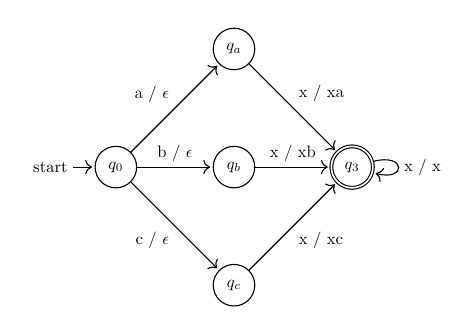
\begin{tikzpicture}[shorten >=1pt, node distance=1.5cm, on grid,
      auto, scale=0.6, every node/.style={scale=0.6}
  ] 
    \node[state,initial] (q_0)   {$q_0$}; 
    \node[state] (q_b) [right=of q_0] {$q_b$}; 
    \node[state] (q_a) [above=of q_b] {$q_a$}; 
    \node[state] (q_c) [below=of q_b] {$q_c$}; 
    \node[state, accepting] (q_1) [right=of q_b] {$q_3$};
    \path[->] 
    (q_0) edge node {a / $\epsilon$} (q_a)
          edge node {b / $\epsilon$} (q_b)
          edge node [below left] {c / $\epsilon$} (q_c)
    (q_a) edge node {x / xa} (q_1)
    (q_b) edge node {x / xb} (q_1)
    (q_c) edge node [below right] {x / xc} (q_1)
    (q_1) edge [loop right] node {x / x} (q_1)
          ;
  \end{tikzpicture}
  \ \ \ \ 
  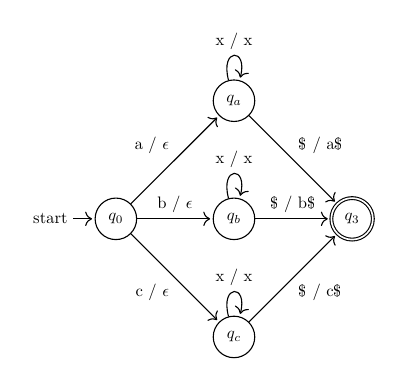
\begin{tikzpicture}[shorten >=1pt, node distance=1.5cm, on grid,
      auto, scale=0.6, every node/.style={scale=0.6}
  ] 
    \node[state,initial] (q_0)   {$q_0$}; 
    \node[state] (q_b) [right=of q_0] {$q_b$}; 
    \node[state] (q_a) [above=of q_b] {$q_a$}; 
    \node[state] (q_c) [below=of q_b] {$q_c$}; 
    \node[state, accepting] (q_1) [right=of q_b] {$q_3$};
    \path[->] 
    (q_0) edge node {a / $\epsilon$} (q_a)
          edge node {b / $\epsilon$} (q_b)
          edge node [below left] {c / $\epsilon$} (q_c)
    (q_a) edge node {\$ / a\$} (q_1)
          edge [loop above] node {x / x} (q_a)
    (q_b) edge node {\$ / b\$} (q_1)
          edge [loop above] node {x / x} (q_b)
    (q_c) edge node [below right] {\$ / c\$} (q_1)
          edge [loop above] node {x / x} (q_c)
          ;
  \end{tikzpicture}
\end{frame}

\begin{frame}[fragile]{Automata -- Invariance under order}
  Theorem: Given a deterministic automata $M$, we can check if $M$
  is invariant under the order of its input
  in time $O(|\Sigma|^2|M|\log(|\Sigma||M|))$.
  \vspace{0.3in}

  Proof:
  \begin{itemize}
    \item Construct the machines $M_{swap}$ and $M_{rot}$ by
      composing $M$ with those machines
    \begin{itemize}
      \item Requires $O(|\Sigma||M|)$ states
    \end{itemize}
    \item Check if $L(M_{swap}) = L(M) = L(M_{rot})$
    \begin{itemize}
      \item E.g. by state minimization in time $O(n|\Sigma| \log n)$
    \end{itemize}
  \end{itemize}
\end{frame}

\begin{frame}[fragile]{Binary Search Trees}
  \begin{itemize}
    \item For lists, two simple permutations generated all permutations
    \item Goal: similar permutations for BSTs
  \end{itemize}
\end{frame}

\begin{frame}[fragile]{Binary Search Trees}
  \begin{columns}
    \begin{column}{0.4\textwidth}
      \qroofx=2
      \qroofy=1
      \Tree [.b [.a \qroof{LL}. \qroof{LR}. ] \qroof{R}. ]
    \end{column}
    \begin{column}{0.1\textwidth}
      $\xmapsto{\mathrm{rotate}}$
    \end{column}
    \begin{column}{0.4\textwidth}
        \qroofx=2
        \qroofy=1
        \Tree [.a \qroof{LL}. [.b \qroof{LR}. \qroof{R}. ]  ]
    \end{column}
  \end{columns}
  \vfill
  \begin{columns}
    \begin{column}{0.45\textwidth}
      \qroofx=2
      \qroofy=1
      \Tree [.c [.a \qroof{LL}. [.b \qroof{LRL}. \qroof{LRR}. ]] \qroof{R}. ]
    \end{column}
    \begin{column}{0.1\textwidth}
      $\xmapsto{\mathrm{flatten}}$
    \end{column}
    \begin{column}{0.45\textwidth}
        \qroofx=2
        \qroofy=1
        \Tree [.c [.b [.a \qroof{LL}. \qroof{LRL}. ] \qroof{LRR}. ] \qroof{R}. ]
    \end{column}
  \end{columns}
  \vfill
\end{frame}

\begin{frame}[fragile]{Binary Search Trees}
  It suffices to show
  \begin{itemize}
    \item Every tree can be transformed into a ``normal form'' (i.e. list)
    \item Every operation is reversable
  \end{itemize}
\end{frame}

\begin{frame}[fragile]{Binary Search Trees -- Proof by example}
  \begin{itemize}
    \item Every tree can be transformed into a ``normal form'' (i.e. list)
  \end{itemize}

  \only<1-2>{
    \Tree [.7 [.3 [.2 1 $\e$ ] [.5 4 6 ]] [.9 8 $\e$ ]]
  }
  \only<2>{
    $\xmapsto{\mathrm{rotate}^{-1}}$
  }
  \only<2-3>{
    \Tree [.9 [.7 [.3 [.2 1 $\e$ ] [.5 4 6 ]] 8 ] $\e$ ]
  }
  \only<3>{
    $\xmapsto{\mathrm{flatten}}$
  }
  \only<3-4>{
    \Tree [.9 [.8 [.7 [.3 [.2 1 $\e$ ] [.5 4 6 ]] $\e$ ] $\e$ ] $\e$ ]
  }
  \only<4>{
    $\xmapsto{\mathrm{rotate}}$
  }
  \only<4-5>{
    \Tree [.8 [.7 [.3 [.2 1 $\e$ ] [.5 4 6 ]] $\e$ ] 9 ]
  }
  \only<5>{
    $\xmapsto{\mathrm{rotate}}$
  }
  \only<5-6>{
    \Tree [.7 [.3 [.2 1 $\e$ ] [.5 4 6 ]] [.8 $\e$ 9 ] ]
  }
  \only<6>{
    $\xmapsto{\mathrm{flatten}}$
  }
  \only<6-7>{
    \Tree [.7 [.5 [.3 [.2 1 $\e$ ] 4 ] 6 ] [.8 $\e$ 9 ] ]
  }
  \only<7>{
    $\xmapsto{\mathrm{flatten}}$
  }
  \only<7-8>{
    \Tree [.7 [.6 [.5 [.3 [.2 1 $\e$ ] 4 ] $\e$ ] $\e$ ] [.8 $\e$ 9 ] ]
  }
  \only<8>{
    $\xmapsto{\mathrm{rotate}}$
  }
  \only<8-9>{
    \Tree [.6 [.5 [.3 [.2 1 $\e$ ] 4 ] $\e$ ] [.7 $\e$ [.8 $\e$ 9 ] ]]
  }
  \only<9>{
    $\xmapsto{\mathrm{rotate}}$
  }
  \only<9-10>{
    \Tree [.5 [.3 [.2 1 $\e$ ] 4 ] [.6 $\e$ [.7 $\e$ [.8 $\e$ 9 ] ]]]
  }
  \only<10>{
    $\xmapsto{\mathrm{flatten}}$
  }
  \only<10-11>{
    \Tree [.5 [.4 [.3 [.2 1 $\e$ ] $\e$ ] $\e$ ] [.6 $\e$ [.7 $\e$ [.8 $\e$ 9 ] ]]]
  }
  \only<11>{
    $\xmapsto{\mathrm{rotate}}$
  }
  \only<11-12>{
    \Tree [.4 [.3 [.2 1 $\e$ ] $\e$ ] [.5 $\e$ [.6 $\e$ [.7 $\e$ [.8 $\e$ 9 ] ]]]]
  }
  \only<12>{
    $\xmapsto{\mathrm{rotate}}$
  }
  \only<12-13>{
    \Tree [.3 [.2 1 $\e$ ] [.4 $\e$ [.5 $\e$ [.6 $\e$ [.7 $\e$ [.8 $\e$ 9 ] ]]]]]
  }
  \only<13>{
     $\xmapsto{\mathrm{rotate}}$
  }
  \only<13-14>{
    \Tree [.2 1 [.3 $\e$ [.4 $\e$ [.5 $\e$ [.6 $\e$ [.7 $\e$ [.8 $\e$ 9 ] ]]]]]]
  }
  \only<14>{
    \hspace{-0.5in} $\xmapsto{\mathrm{rotate}}$
  }
  \only<14-15>{
    \Tree [.1 $\e$ [.2 $\e$ [.3 $\e$ [.4 $\e$ [.5 $\e$ [.6 $\e$ [.7 $\e$ [.8 $\e$ 9 ] ]]]]]]]
  }
\end{frame}

% Maybe swap the code example for a list function
% Save this for the paper
\begin{frame}[fragile]{Checking BST code}
  \begin{itemize}
    \item Goal: write a secondSmallest function on BSTs
  \end{itemize}
  secondSmallest$\Bigg($\hspace{-1in}\Tree [.b [.a $\e$ $\e$ ] \qroof{R}. ]$\Bigg)$ = b
  \vfill
  secondSmallest$\Bigg($\hspace{-0.7in}\Tree [.a $\e$ \qroof{R}. ]$\Bigg)$ = smallest(R)
  \vfill
  (more cases)
\end{frame}

\begin{frame}[fragile]{Checking BST code}
  \begin{itemize}
    \item One case of checking invariance under rotation:
  \end{itemize}
  \begin{align*}
    secondSmallest\Bigg(\Tree [.b [.a $\e$ $\e$ ] \qroof{R}. ] \Bigg) 
      & = &
    secondSmallest\Bigg(\Tree [.a  $\e$ [.b $\e$ \qroof{R}. ]] \Bigg) 
     \\ 
    b
      & = &
    smallest\Bigg(\Tree [.b $\e$ \qroof{R}. ] \Bigg) 
  \end{align*}

\end{frame}

\begin{frame}[fragile]{More General Procedure}
  Invariance of a program $P : T\to Z$
  relative to a function $f : T \to T'$
  \begin{itemize}
    \item E.g. $f : BST \to List$
  \end{itemize}
  \vfill
  Observation:
  The following are equivalent:
  \begin{itemize}
    \item $f(x) = f(y) \implies P(x) = P(y)$
    \item There exists a program $\widetilde{P} : T'\to Z$
      such that $P = \widetilde{P} \circ f$
  \end{itemize}

  \[
    \begin{tikzcd}
      T \arrow{rr}{P} \arrow{rd}{f} &   & Z \\
      & T' \arrow[dashed]{ru}{\widetilde{P}} &   \\
    \end{tikzcd}
  \]
\end{frame}

\begin{frame}[fragile]{More General Procedure}
  \begin{itemize}
    \item Idea: Synthesize a witness to the invariance
    \begin{itemize}
      \item A function $\widetilde{P} : T' \to Z$
    \end{itemize}
    \item $P$ and $f$ provide a \emph{full specification} of $\widetilde{P}$
    \item Counterexample guided inductive synthesis
  \end{itemize}

  \[
    \begin{tikzcd}
      T \arrow{rr}{P} \arrow{rd}{f} &   & Z \\
      & T' \arrow[dashed]{ru}{\widetilde{P}} &   \\
    \end{tikzcd}
  \]
\end{frame}

\begin{frame}[fragile]{More General Procedure}
  \tikzstyle{process} = [rectangle, minimum width=3cm, minimum height=1cm,
    text centered, draw=black, fill=orange!30,
    text width=10em ]
  \tikzstyle{smallprocess} = [rectangle, minimum width=3cm, minimum height=1cm,
    text centered, draw=black, fill=orange!30,
    text width=6em ]
  \tikzstyle{io} = [rectangle, rounded corners,
    minimum width=3cm, minimum height=1cm,
    text centered, draw=black, fill=blue!30]
  \tikzstyle{arrow} = [thick,->,>=stealth]

  \begin{tikzpicture}[node distance=2cm, scale=0.8, every node/.style={scale=0.8}]
    \node (start) [io] {
      Input $P$ and $f$.
      Let $E = \{ \}$.
    };
    \node (synth) [process, below of=start, yshift=-0.5cm] {
      Synthesize a program $\widetilde{P} : T' \to Z$
      given examples $\{ (f(x), P(x)) | x\in E \}$
    };
    \node (verify) [process, right of=synth, xshift=4cm] {
      Verify whether $\widetilde{P}\circ f$
      is equivalent to $P$
    };
    \node (yes) [io, above of=verify] {
      return YES
    };
    \node (check) [process, below of=verify, yshift=-1cm] {
      Check if there are any $x\in E$ such that
      $f(x)=f(x_0)$, yet $P(x) \ne P(x_0)$
    };
    \node (no) [io, below of=check, yshift=-0.5cm] {
      return NO
    };
    \node (add) [smallprocess, below of=synth, yshift=-1cm] {
      Add $x_0$ to the example set $E$
    };

    \draw [arrow] (start) -- (synth);
    \draw [arrow] (synth) -- (verify);
    \draw [arrow] (verify) --
      node[anchor=west, text width=6cm] {No, with \\ counterexample $x_0\in T$}
      (check);
    \draw [arrow] (verify) --
      node[anchor=west, text width=6cm] {Yes, equivalent}
      (yes);
    \draw [arrow] (check) --
      node[anchor=north, text width=2cm, text centered] {No, $x$ does not exists}
      (add);
      \draw [arrow] (add) -- (synth);
    \draw [arrow] (check) --
      node[anchor=west, text width=6cm] {Yes, $x$ exists}
      (no);
  \end{tikzpicture}
\end{frame}

\begin{frame}[fragile]{More General Procedure}
  asdf
\end{frame}



\end{document}

% \begin{frame}[fragile]{Multicolumn Example}
%   \begin{columns}
%     \begin{column}{0.5\textwidth}
%       Hello
%     \end{column}
%     \begin{column}{0.5\textwidth}  %%<--- here
%       \begin{flushright}
%       image
%       \end{flushright}
%     \end{column}
%   \end{columns}
% \end{frame}

% \begin{frame}[fragile]{The Code Topology $T(1,1,1)$}
%   View codewords as a grid
%   \vfill
%   \begin{tabular}{c c c >{\columncolor[rgb]{.8,.8,1}}c | c}
%     $x_{1,1}$ & $x_{1,2}$ & $x_{1,3}$ & $x_{1,1} + x_{1,2} + x_{1,3}$ \\
%     $x_{2,1}$ & $x_{2,2}$ & \cellcolor[rgb]{1,0,0}$y$ & $x_{2,1} + x_{2,2} + y$ \\
%     \rowcolor[rgb]{.8,.8,1}
%     $x_{1,1}+x_{2,1}$ & $x_{1,2}+x_{1,2}$ & $x_{1,3}+y$ & (*) & (column parities)\\
%     \hline
%     & & & (row parities)
%   \end{tabular}
%   \vfill
%   Parities for correlated failures
%   \hfill
%   \emphasizeWhen{2}{
%     Maximize Recoverability
%   }

%   $(*) = \sum_{i,j} x_{i,j} $
%   \hfill
%   \emphasizeWhen{2}{
%     $y = \sum_{i,j} \gamma_{i,j} x_{i,j}$
%   }

%   \hfill
%   \emphasizeWhen{2}{
%     Global ``backup" parity
%   }

% \end{frame}
